\chapter{Web Platform Flows}

The previous chapters explain the logic behind the components of the web platform. In this chapter, some of the web platform's flows are explained, either from the user's perspective or from the system's perspective. Some flows presented below are subject to change as the application evolves.

\section{Reading courses}

\begin{figure}[h]
    \centering
    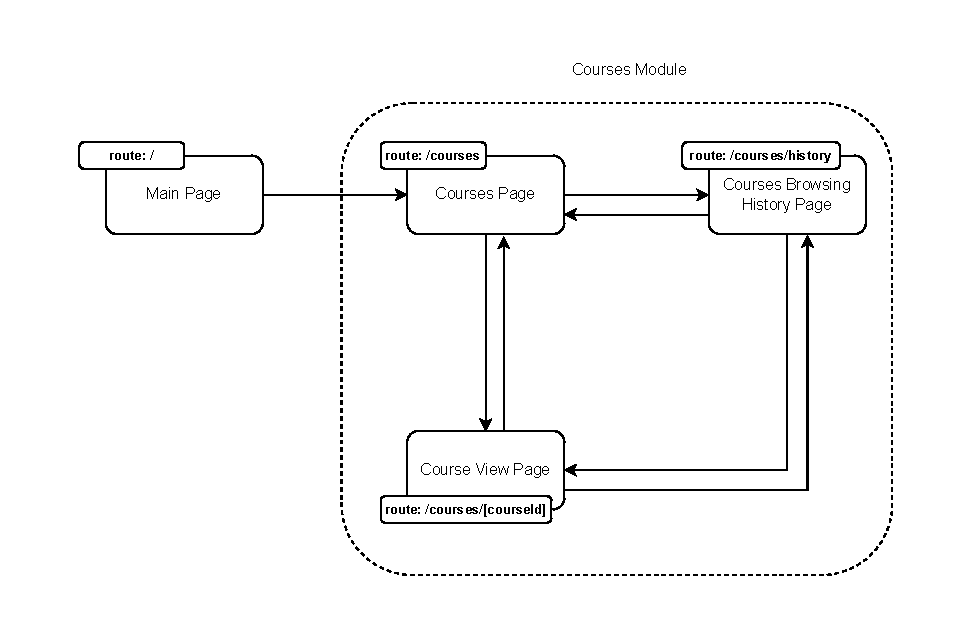
\includegraphics{images/course-reading-flow.pdf}
    \caption{User Flow - Reading courses}
    \label{fig:course-reading-flow}
\end{figure}

\newpage
\noindent Referring to the \textbf{main page} of the web platform as the starting point, the user can start reading courses by either clicking redirection links on the main page or by manually entering the course URLs. From Figure \ref{fig:course-reading-flow}, it can be observed that the user can navigate through the pages without being authenticated.
\\\\
\noindent The \textbf{courses page} is a list of all the courses available on the platform. From here, the user can click on a course from the list and be redirected to that course's view page. The route for the courses page can also receive the query parameter \textbf{search}, which will filter the courses based on the search query.
\\\\
\noindent The \textbf{courses browsing history page} is a list of all the courses that the user has visited. Selecting a course on this page will redirect to its view page.
\\\\
\noindent Both the courses page and the courses browsing history page are accessible through the global courses module navbar. Users can quickly navigate to these pages from any page that is part of the courses module.

\section{Manage courses}

\begin{figure}[h]
    \centering
    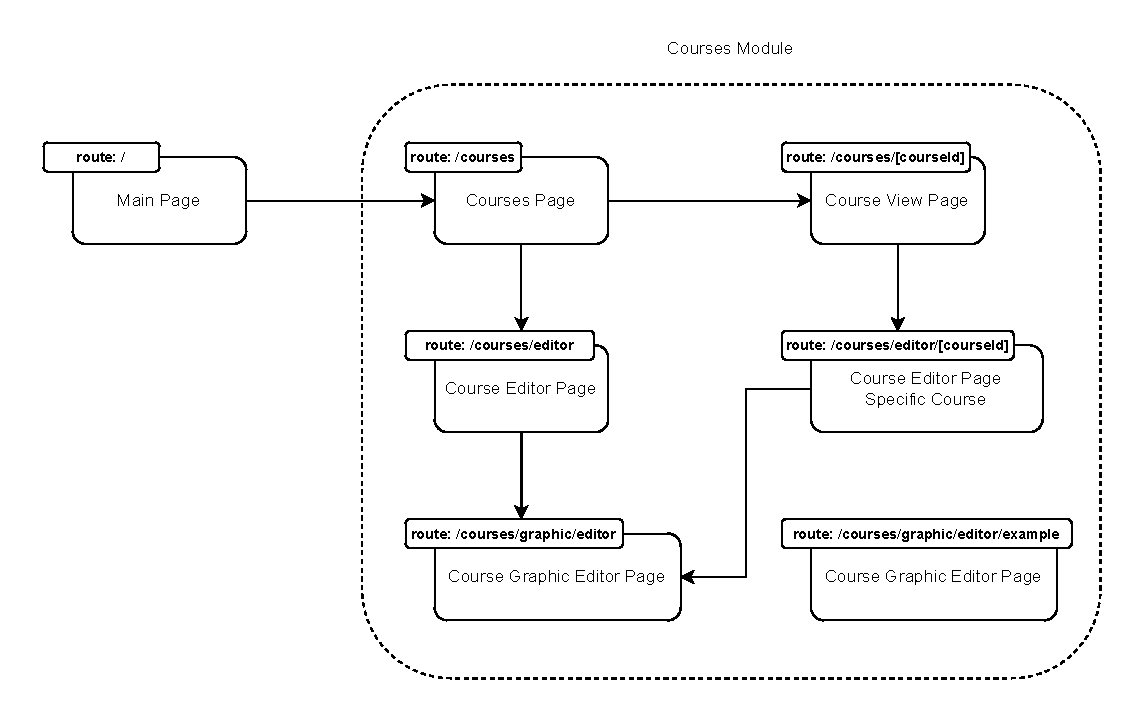
\includegraphics[scale=0.85]{images/course-manage-flow.pdf}
    \caption{User Flow - Manage courses}
    \label{fig:course-manage-flow}
\end{figure}

\newpage
\noindent All the editors are accessible even for unauthenticated users. The \textbf{course editor} is a page where a JSON editor is displayed, along with a live preview of how the editor's content will be rendered. It is accessible via the global courses module navbar. An unauthenticated user can play around in this editor and copy or download the JSON when they are satisfied with the result. In the case of authenticated users who also have the role of \textbf{Course Manager}, they can save the course to the database as a new course.
\\\\
\noindent The \textbf{course editor for a specific course} is the same as the course editor, but it is pre-filled with the content of the course given as a path variable. This editor is accessible from the course view page, by clicking the \textbf{Open in Editor} button. If the user is, once again, authenticated and has the role of \textbf{Course Manager}, they can save the course to the database as an update to the existing course. Unauthenticated users can still access a specific course editor, but they cannot save the course to the database. They are allowed because the official courses can be great examples of how to create their own courses.
\\\\
\noindent The graphic editor is a standalone editor that is accessible via the route mentioned in Figure \ref{fig:course-manage-flow} or via widgets from the course JSON editor. The difference between the two methods is that the first one opens an empty editor while the second method uses localStorage to pre-fill the graphic editor with one taken from the clicked widget. This page is the same for both authenticated and unauthenticated users, as the graphic needs to be copy-pasted into the course's content to be saved.
\\\\
\noindent The \textbf{course graphic editor page} from Figure \ref{fig:course-manage-flow} that is not connected to any other page can only be accessed via the route and contains a pre-filled example graphic that can still be edited.

\section{User authentication}

\noindent Authenticating the user is currently used only for allowing some people to manage the courses. The authentication flow is presented in Figure \ref{fig:user-auth-flow}.
\\\\
\noindent To start the authentication flow, you obviously need to do \textbf{step 1}, by entering the login page. The login page is accessible via the global navbar, by clicking the \textbf{Login} button. You can also manually navigate to the login page by entering the URL, but that would redirect to the main page.
\\\\
\noindent \textbf{Step 2} is to select the authentication provider. Currently, the only authentication providers usable are Discord and GitHub. Selecting a provider will trigger a redirection to one of \textbf{NextAuth's routes}, where the OAuth2 process will be started.
\\\\
\noindent \textbf{Step 3} is redirecting to the OAuth2 provider associated with the client registration selected. The user will be prompted to log in to the provider and authorize the web platform to access their account. After the user has authorized the web platform, they will be redirected back to the web platform in \textbf{step 4}.
\\\\
\noindent Based on the response from the OAuth2 provider, the NextAuth callback will decide if the user is authenticated or not. If an error has occurred, the user is redirected to the login page (taking the \textbf{5 error step}). If the user is authenticated with the OAuth2 server, the second part of the authentication process will be started. Following the \textbf{5 success step}, the Spring Boot authorization server will be called to generate a JWT token for the user. This token will be stored in the user's browser and will be used to authenticate the user in the future.
\\\\
\noindent The response, represented by \textbf{step 6}, will be processed by another NextAuth callback, which will either create a session for the user and redirect them to the page where the authentication flow started (\textbf{step 7 success}) or redirect them to the login page with an error message (\textbf{step 7 error}).
\\\\
\noindent Registration is not needed for the web platform, as the users are authenticated via OAuth2 providers. When authenticating the user, the backend auth server is responsible for managing the users and linking providers to the same account based on email.

\begin{figure}[h]
    \centering
    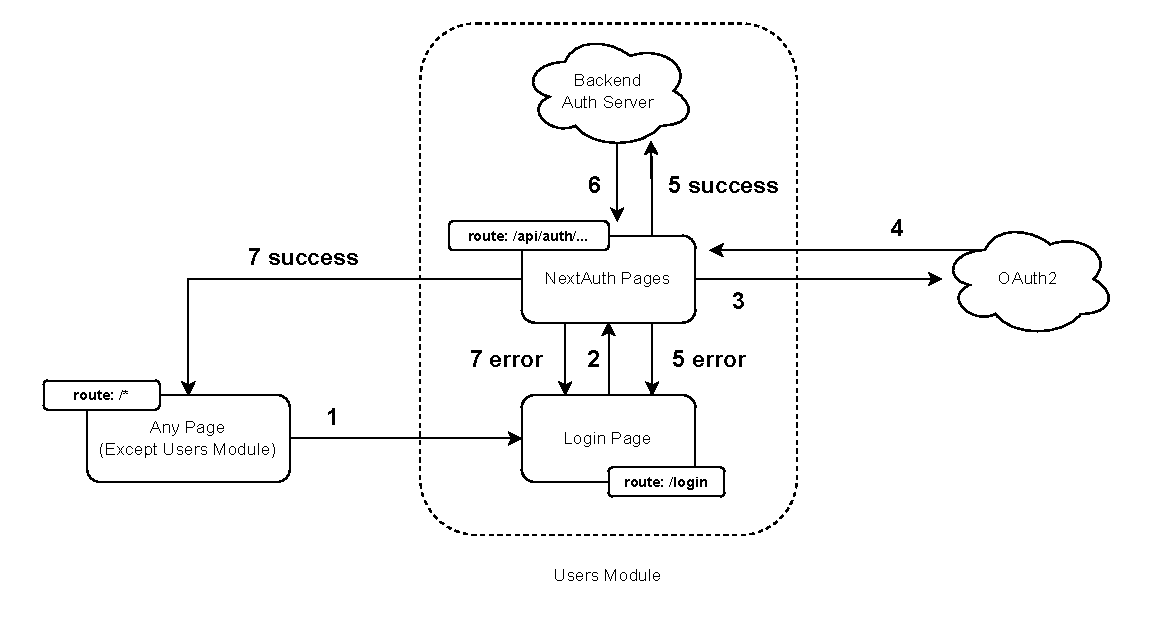
\includegraphics[scale=0.85]{images/user-auth-flow.pdf}
    \caption{User Flow - Authentication}
    \label{fig:user-auth-flow}
\end{figure}

\section{Accessing Resources}

\noindent After the user is authenticated, the session will contain two tokens generated by the authentication server. The first token is the access token, which is used to access protected resources. The second token is the refresh token, which is used to refresh the access token when it expires.
\\\\
\noindent Some resources are protected, while others are public but have protected actions. The public resources of the web platform are the courses, but editing them is a private action. The protected resources are the ones that require the user to be authenticated and have a specific role. The flow for accessing protected resources is presented in Figure \ref{fig:protected-resources-sequence}.

\begin{figure}[h]
    \centering
    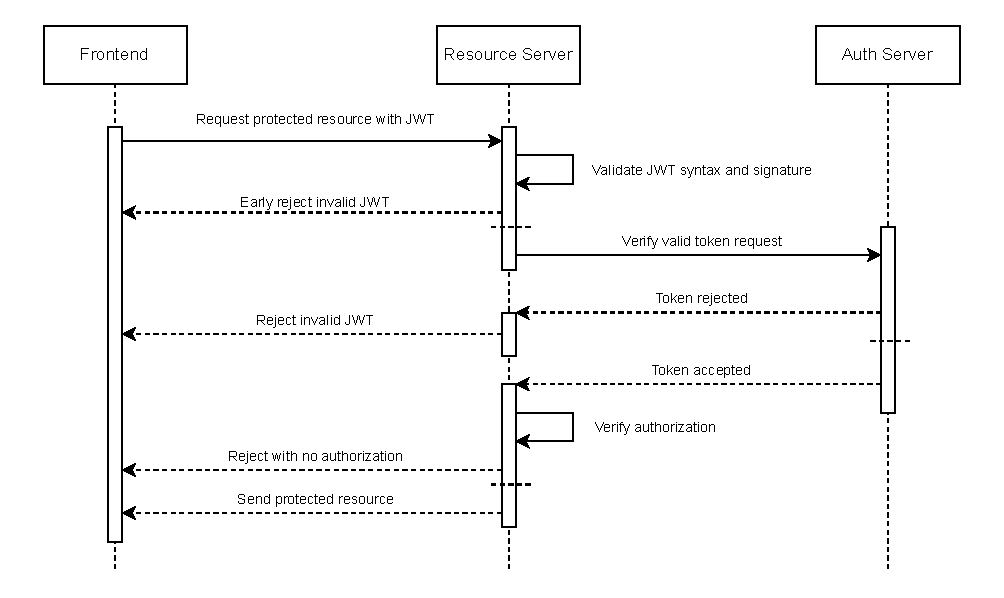
\includegraphics{images/accessing-protected-resources-flow.pdf}
    \caption{Accessing protected resources sequence diagram}
    \label{fig:protected-resources-sequence}
\end{figure}

\noindent Requests from the frontend to access protected resources must be done with an access token, referred to in the Figure as a JWT. If no access token is specified in the request, the resource server will automatically reject the request with a 401 Unauthorized status code. That is only the case for resources that require authentication.
\\\\
\noindent The access token is validated in the second step, basically verifying that the token is properly formatted. This is done to prevent useless requests to the authorization server. If the token is not valid, the resource server will reject the request early with a 401 Unauthorized status code.
\\\\
\noindent To validate the token, the resource server will call the authorization server to check if the token is still valid. It will verify the signature of the token using the secret key of the authorization server. If the token is expired or has been tampered with, the resource server will reject the request with a 401 Unauthorized status code. The authorization server will also reject the token if it has been invalidated inside the database. If the token is valid, the resource server will continue processing the request.
\\\\
\noindent Now that the token is for sure valid, the resource server will check if the user has the required role to access the resource. If the user does not have the required role, the resource server will reject the request with a 403 Forbidden status code. If the user has the required role, the resource server will continue processing the request.
\\\\
\noindent The resource server will finally process the request and return the response to the frontend. The response will contain the requested data or an error message if something went wrong.
\\\\
\noindent The short dotted lines in the Figure represent an alternative flow, taken if the previous action was not already taken. For example, verifying if the token is valid is an alternative if the early reject action was not taken.
\\\\
\noindent Even if the Figure \ref{fig:protected-resources-sequence} presents the flow for accessing protected resources, the same flow applies to protected actions that do not necessarily involve returning data but are modifying it.